
\documentclass[12pt,fleqn,leqno,letterpaper]{article}
\usepackage[utf8]{inputenc}
\usepackage[english]{babel}

\usepackage{hyperref}
\usepackage{graphicx}
\usepackage{minted}

\include{preamble}


\title{Assignment x}
\author{Anders L. Hurum\\
    \small{Development of Real-Time Systems}\\
    \small{EIT Digital}\\
    \small{\texttt{andershurum@gmail.com}}
}
\date{September 17, 2017}

\begin{document}


    \maketitle

    \begin{abstract}
        
        The xx assignment for the course consisted of . \\ \\
        For more details on the assignment, see the \texttt{assignment\_x.md} document 
        in the repository at github. \\
        
        \url{http://github.com/peakbreaker/tuts\_FreeRTOS}

    \end{abstract}

    \newpage

    \section*{Code}

        Main:

        \begin{minted}{c}
            int main(void)
            {
                
            }
        \end{minted}

        The ... task:

        \begin{minted}{c}
            
        \end{minted}

        To accomplish the assignment I ..
    \newpage
    \section*{Results}

        The resulting output from the program were as follows : \\

        \begin{figure}[h]
            \centering
            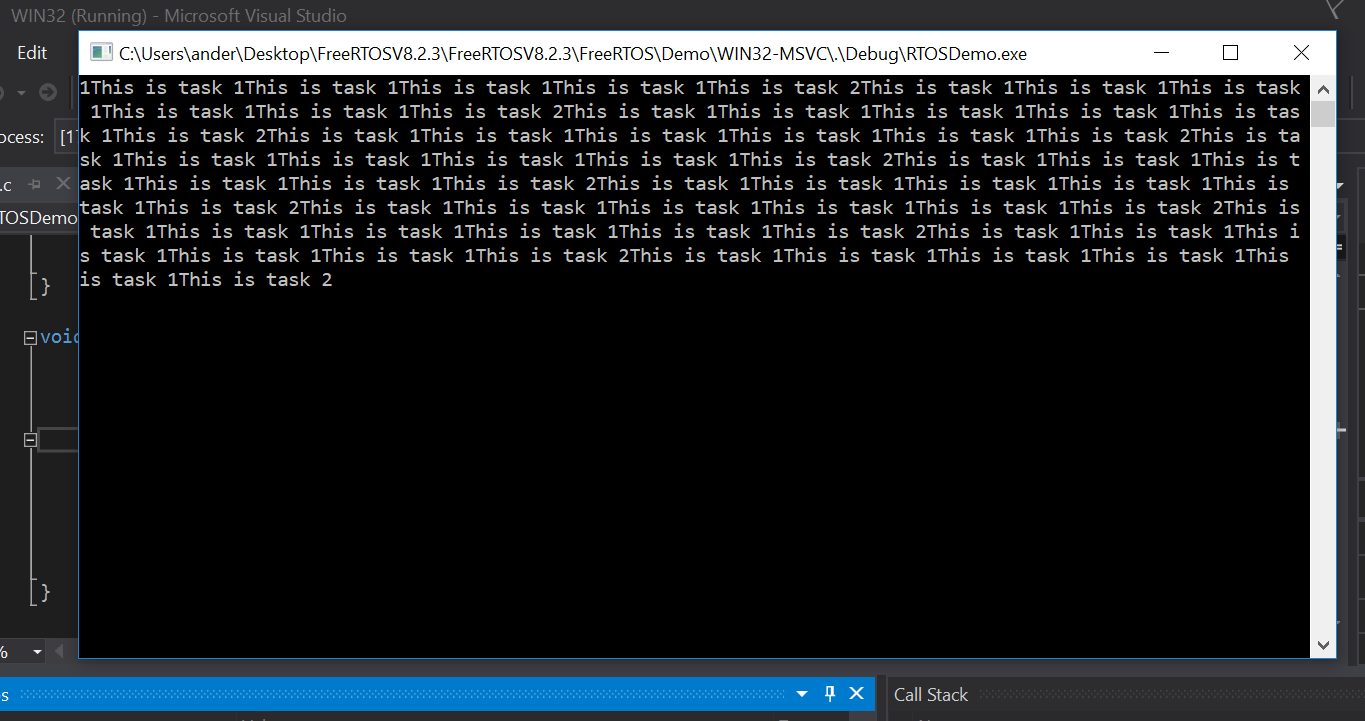
\includegraphics[width=\textwidth]{Debug.png}
            \caption{Debug output}
            \label{figure:debug}
        \end{figure}

        As the output shows, \\
        
        The repository for the entire assignment can be found at my github : \\
        
        \url{http://github.com/peakbreaker/tuts\_FreeRTOS}

    \end{document}